%%% CAPITOLO 2
%%% STRATEGIE DI TRADING E BACKTESTING

\section{Strategie di trading e backtesting}

Il backtesting ci permette di valutare la performance di una strategia di trading utilizzando
indicatori euristici o tecnici e applicandoli a dati storici.

Nel contesto di questo progetto, è stato creato un algoritmo di trading usando la tecnica BB

\subsection{Strategia buy/sell mediante Bollinger's Bands}

Le bande di Bollinger sono un metodo statistico per derivare informazioni sul prezzo e volatilità di un asset
nel tempo.

Per ottenere le bade di Bollinger abbiamo bisogno di calcolare la media mobile e la deviazione standard della serie
temporale, utilizzando una finestra specifica (tipicamente 20 giorni). Successivamente dobbiamo importare la banda
superiore/inferiore a $K$ volte (tipicamente 2) la deviazione standard mobile sopra o sotto la media mobile.

Per la strategia di trading scelta è stata impostata come finestra 20 giorni e come fattore di deviazione $2$.

\pagebreak

\subsection{Backtesting su titolo Meta (FB)}

Per effettuare il backtesting della strategia scelta, è stato preso in considerazione il titolo Meta (FB) nell'anno
2020, si può trovare il grafico a pagina \ref{fig:fb_backtest}.

\begin{figure}[ht]
    \centering
    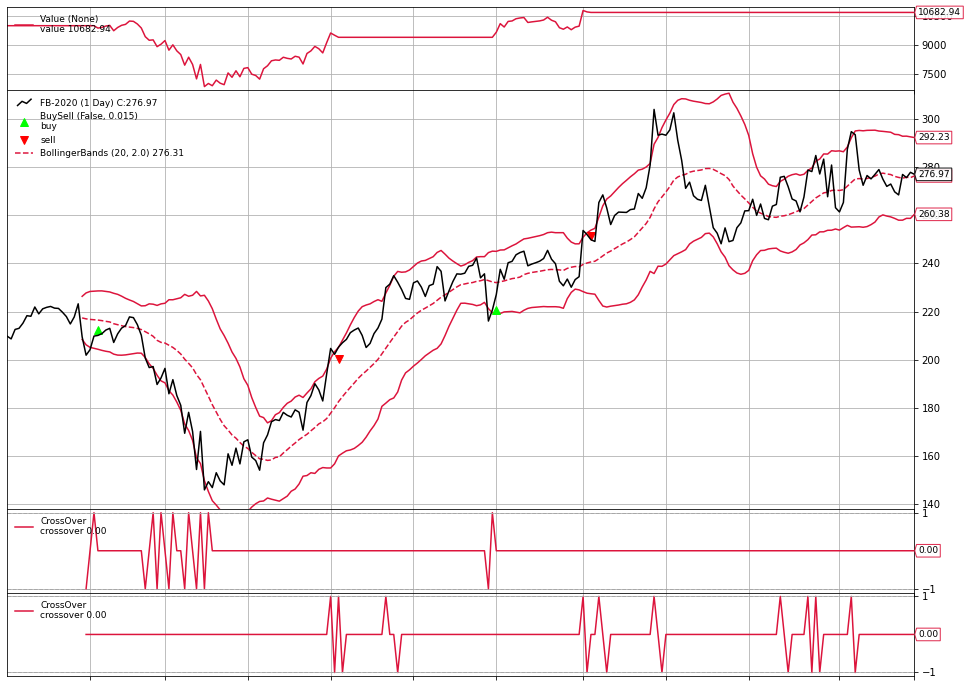
\includegraphics[width=1\textwidth]{fb_backtrack.png}
    \caption{Backtesting della strategia BB su FB}
    \label{fig:fb_backtest}
\end{figure}

\begin{figure}[ht]
    \centering
    \begin{minipage}{.6\textwidth}
        \centering
        \vspace{1.27cm}
        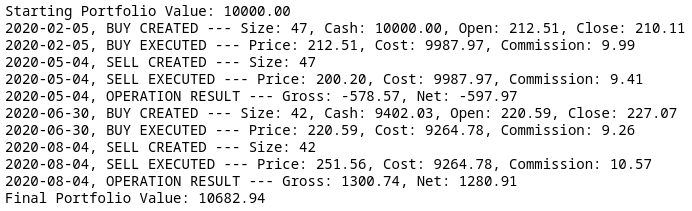
\includegraphics[width=.8\linewidth]{fb_backtrack_buy_sell.png}
        \captionof{figure}{backtrader log for FB}
        \label{fig:fb_backtr_log}
    \end{minipage}%
    \begin{minipage}{.4\textwidth}
        \centering
        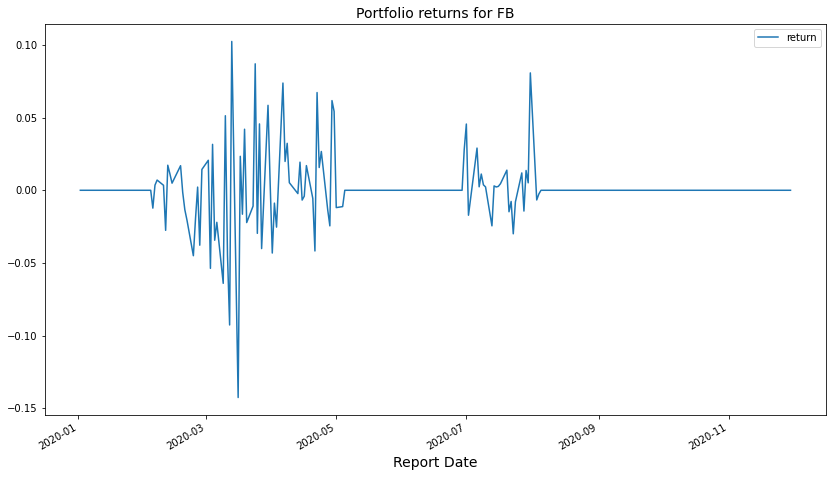
\includegraphics[width=1\linewidth]{fb_backtrack_ret.png}
        \captionof{figure}{Backtesting portfolio returns}
        \label{fig:fb_backtr_ret}
    \end{minipage}
\end{figure}

Dai log di \verb|backtrader| a figura \ref{fig:fb_backtr_log} si può vedere come la strategia è riuscita ad avere un profitto,
passando da $10000.00\$$ a $10682,94\$$ marcando un profitto di $682,94\$$ nel corso di un anno.